\documentclass[12pt]{article}

\usepackage{scicite,times,graphicx,float,hyperref}
\usepackage[skip=0pt]{caption}
\usepackage[utf8]{inputenc}
\usepackage{enumitem}
\usepackage{booktabs}
\usepackage{multicol}

\topmargin -1.0cm
\oddsidemargin 0.0cm
\textwidth 16cm 
\textheight 23cm
\footskip 1.0cm

\newenvironment{sciabstract}{%
\begin{quote} \bf}
{\end{quote}}

\newcounter{lastnote}
\newenvironment{scilastnote}{%
  \setcounter{lastnote}{\value{enumiv}}%
  \addtocounter{lastnote}{+1}%
  \begin{list}%
  {\arabic{lastnote}.}
  {\setlength{\leftmargin}{.22in}}
  {\setlength{\labelsep}{.5em}}
}
{\end{list}}

\title{Simulation of a Scientific Computation Platform\\With a Focus on Quality Attributes} 

\author
{Filipe Pires [85122], João Alegria [85048]\\
\\
Software Architecture\\
\normalsize{Department of Electronics, Telecommunications and Informatics}\\
\normalsize{University of Aveiro}\\
} 

\date{\today{}}

%%%%%%%%%%%%%%%%% END OF PREAMBLE %%%%%%%%%%%%%%%%

\begin{document}

\baselineskip18pt

\maketitle

\section*{Introduction} %%%%%%%%%%%%%%%%%%%%%%%%%%%%%%%%%%%%%%%%%%%%%%%%%%%%%%%%%%%%%%%%%%%%%%%%%%%%%%%%%%%%%%%%%%%%%%%%%%%%%%%%%%%%%%%%%%%%%%%%%%%%%%%%%%%%%%%%

This report aims to describe the work developed for the third and final assignment of the course of 'Software Architecture', focused on a platform that accepts 
and processes computational services requested by the scientific community. 

The aim of the assignment was to design and develop a software architecture relying on four of the most relevant quality attributes:
performance, availability, scalability and usability.
Playing the role of software architects, we came up with the solution for an infrastructure for our stakeholder.
The platform here presented is capable of deploying a cluster of servers monitored by a tactic entity and whose requests from clients are distributed by a load balancer.
Although the cluster is locally simulated, the configuration is done so that it is possible to deploy in a distributed environment.

So in this report we present the architecture of our solution, justifying design decisions according to what we learned and found to be most suitable for our use case.
We also mention how the work was distributed amongst the authors.

All code developed is publicly accessible in our GitHub repository:

\url{https://github.com/FilipePires98/AS/}

% \vspace{-10pt}
% \begin{itemize}[noitemsep]
%   \item Prepare - the selected farmers move to a Standing Area, ready for orders.
%   \item Start - the actual simulation begins and farmers start moving.
%   \item Collect - farmers collect corn cobs from the Granary (where the cobs initially are).
%   \item Return - farmers return to the Storehouse with the collected corn cobs.
%   \item Stop - farmers stop whatever they are doing and return to the Storehouse.
%   \item Exit - simulation ends and the program closes.
% \end{itemize}
% \vspace{-10pt}

% \begin{figure}[H]
%   \centering
%   \begin{minipage}{\textwidth}
%     \centering
%     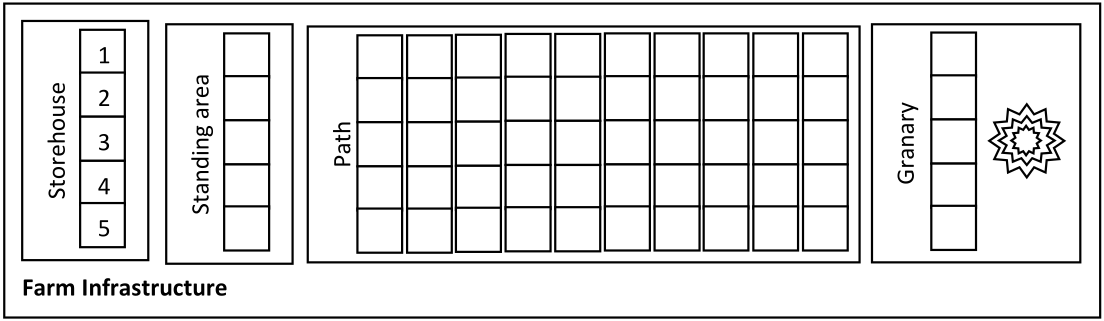
\includegraphics[width=\linewidth]{img/Design_FI.png}
%   \end{minipage}%
%   \caption{Visual representation of the farm, taken from \cite{assign}.}
%   \label{Design_FI}
% \end{figure} 

%\texttt{java -cp <userdir>/build/classes fi.FarmInfrastructure}

\newpage
\section{Scientific Computation and Custom Systems} %%%%%%%%%%%%%%%%%%%%%%%%%%%%%%%%%%%%%%%%%%%%%%%%%%%%%%%%%%%%%%%%%%%%%%%%%%%%%%%%%%%%%%%%%%%%%%%%%%%%%%%%%%%%%%%%%%%%%

Applied computer science and mathematics often use advanced computing capabilities to understand and solve complex problems.
In practical use, computational science is typically the application of computer simulation and other forms of computation to tackle problems in various 
scientific disciplines.
Scientists and engineers develop computer programs that model systems being studied and run these programs with various sets of input parameters.
In some cases, these models require massive amounts of calculations and are often executed on supercomputers or distributed computing platforms.

This project does not describe one of these models, rather it is about the development of an infrastructure capable of supporting such computationally demanding tasks.
The adopted strategy was of coordinating a cluster of processing servers.
The following tactics were selected to be implemented:
\vspace{-10pt}
\begin{itemize}[noitemsep]
  \item Computation Replicas - requests must be fairly distributed amongst the servers.
  \item Concurrency - each request runs on its own thread in a server.
  \item Redundancy - in case a server goes down, requests should be reallocated.
  \item Monitor - everything must be supervised, from the cluster's status, to the clients' identification and request treatment.
  \item Horizontal scalability - new servers can be deployed whenever necessary.
\end{itemize}
\vspace{-10pt}

\subsection{The Scenario} %%%%%%%%%%%%%%%%%%%%%%%%%%%%%%%%%%

In order to test the application of the infrastructure on a scientific problem, an example scenario was adopted: the calculation of the mathematical constant $\pi$ (pi).
Being an irrational number, $\pi$ cannot be expressed as a common fraction and its decimal representation never ends and never settles into a permanently repeating pattern.
Nevertheless, in the 21st century, mathematicians and computer scientists have pursued new approaches that, when combined with increasing computational power, 
extended the decimal representation of $\pi$ to many trillions of digits \cite{pisky}.
The primary motivation for these computations is as a test case to develop efficient algorithms to calculate numeric series, as well as the quest to break records.

The most commonly adopted forms of calculating $\pi$ are the iterative algorithms \cite{jorg}.
In order to only focus on the infrastructure's implementation, while simulating the actual implementation of the iterative algorithms, a control variable 
corresponding to the number of iterations to be used on the calculation was introduced to regulate servers' response times. 

\subsection{The Messages} \label{messages} %%%%%%%%%%%%%%%%%

One of the fundamental constraints applied to our implementation was related to communications.
Each individual server is launched as an independent process.
This is also true for each individual client.
The orchestrator runs in an independent process as well, serving as both a load balancer and a tactic monitor - although these two are built as separate entities.
So in order for entities to communicate with each other, the TCP/IP socket technology was made a requirement. 

For simplicity, only two service message types were defined:
\vspace{-10pt}
\begin{itemize}[noitemsep]
  \item Request: $|$ \texttt{clientID} $|$ \texttt{requestID} $|$ \texttt{01} $|$ \texttt{\# iterations} $|$
  \item Reply: $|$ \texttt{serverID} $|$ \texttt{clientID} $|$ \texttt{requestID} $|$ \texttt{02} $|$ \texttt{\# iterations} $|$ \texttt{pi} $|$
\end{itemize}
\vspace{-10pt}
In them are the following parameters: 
\texttt{clientID}, a positive integer that uniquely identifies a client machine; 
\texttt{serverID}, a positive integer that uniquely identifies each physical server in the cluster;
\texttt{requestID}, a positive integer that uniquely identifies a pi calculation request (computed as 1000 $\times$ \texttt{client id} $+$ increment);
\texttt{01} and \texttt{02}, the request and reply codes;
\texttt{\# iterations}, the chosen value for the previously mentioned control variable used to simulate the number of iterations for the computation of pi
(each iteration / cycle corresponds to 1 second);
\texttt{pi}, the computed value of $\pi$.

A few additional message types were added during development for management purposes:
\vspace{-10pt}
\begin{itemize}[noitemsep]
  \item Heartbeat: ..................................
\end{itemize}
\vspace{-10pt}

..............................................................................................

\newpage
\section{System Architecture} %%%%%%%%%%%%%%%%%%%%%%%%%%%%%%%%%%%%%%%%%%%%%%%%%%%%%%%%%%%%%%%%%%%%%%%%%%%%%%%%%%%%%%%%%%%%%%%%%%%%%%%%%%%%%%%%%%%%%%%%%%%%%%%%%%


\subsection{Entities} \label{entitites} %%%%%%%%%%%%%%%%%%%%


\subsection{Components} \label{components} %%%%%%%%%%%%%%%%%


\subsection{User Interface} %%%%%%%%%%%%%%%%%%%%%%%%%%%%%%%%


\section{Architecture Constraints} \label{infrastructure} %%%%%%%%%%%%%%%%%%%%%%%%%%%%%%%%%%%%%%%%%%%%%%%%%%%%%%%%%%%%%%%%%%%%%%%%%%%%%%%%%%%%%%%%%%%%%%%%%%%%%%%%%%


\subsection{Quality Attributes Assurance} %%%%%%%%

\subsection{User Cases Compliance} %%%%%%%%

\newpage
\section{Additional Remarks} %%%%%%%%%%%%%%%%%%%%%%%%%%%%%%%%%%%%%%%%%%%%%%%%%%%%%%%%%%%%%%%%%%%%%%%%%%%%%%%%%%%%%%%%%%%%%%%%%%%%%%%%%%%%%%%%%%%%%%%%%%%%%%%%%%%

\subsection{Documentation} %%%%%%%%%%%%%%%%%%%%%%%%%%%%%%%%%

Our attitude towards the developed code was to ensure it could be applied to other similar scenarios and reused in systems intended to be deployed in real scenarios.
With this in mind, we took great care with regards to code readability.
By maintaining a code style equal throughout the project and defining intuitive and self-explaining variable and method names, we made the code easy to understand
by someone already contextualized with Kafka.

Nevertheless, we wanted to make sure this was also true to someone looking at our project for the first time, so we resorted to the well-known Javadoc
\cite{javadoc} tool to manage all code documentation.
Comments were also added in key points throughout the code, including the scripts.

\subsection{Assignment Contributions} %%%%%%%%%%%%%%%%%%%%%%

As the entire development phase took place in a time where on-site cooperation was not possible, we resorted to online communication platforms to debate decisions
and discuss difficulties.
Team scheduling allowed us to work on the project simultaneously, so no member suffered from unbalanced workloads.
The dimension of the project did not appeal to the usage of repository pull requests and other synchronization tools.
However, each small solution was verified and agreed by both team members.

Having said this, it is difficult to isolate what each member actually implemented, as the influence of both is present in all components.
Nevertheless, one might say that each had stronger responsibilities on a set of project aspects:
Filipe took care of the execution of the individual Java processes and of the Shell scripts, while João developed the Kafka-related classes such as Consumer,
Producer and EntityAction; Filipe developed the Python script for generation of \texttt{CAR.TXT}, while João developed the Shell scripts for Kafka initialization
and deletion; each implemented 2 entities and each wrote a portion of this report; Filipe made sure everything was coherent throughout the report and the code
documentation, while João solved the most critical issues regarding the configuration of the topics.
In terms of work percentage, we believe it was about 50\% for each student.

\newpage
\section*{Conclusions} %%%%%%%%%%%%%%%%%%%%%%%%%%%%%%%%%%%%%%%%%%%%%%%%%%%%%%%%%%%%%%%%%%%%%%%%%%%%%%%%%%%%%%%%%%%%%%%%%%%%%%%%%%%%%%%%%%%%%%%%%%%%%%%%%%%%%%%%%

\begin{thebibliography}{9} %%%%%%%%%%%%%%%%%%%%%%%%%%%%%%%%%%%%%%%%%%%%%%%%%%%%%%%%%%%%%%%%%%%%%%%%%%%%%%%%%%%%%%%%%%%%%%%%%%%%%%%%%%%%%%%%%%%%%%%%%%%%%%%%%%%%%
  \bibliographystyle{Science}

  \bibitem{pisky}
  \textit{Pi in the sky: Calculating a record-breaking 31.4 trillion digits of Archimedes' constant on Google Cloud}.
  \href{https://web.archive.org/web/20191019023120/https://cloud.google.com/blog/products/compute/calculating-31-4-trillion-digits-of-archimedes-constant-on-google-cloud}
  Retrieved May 2020. 

  \bibitem{jorg}
  Arndt, Jorg \& Haenel, Christoph (2006). 
  \textit{Pi Unleashed}, in Springer-Verlag. 
  ISBN 978-3-540-66572-4. 
  Retrieved May 2020. 
  English translation by Catriona and David Lischka.

  % \bibitem{uml}
  %   Object Management Group,
  %   \textit{What is UML},
  %   \url{https://www.uml.org/what-is-uml.htm},
  %   accessed in March 2020.



\end{thebibliography}

\clearpage

\end{document}




















